\documentclass[a4paper,man,natbib]{apa6}

\usepackage{icml2018}
\usepackage[english]{babel}
\usepackage[utf8x]{inputenc}
\usepackage{amsmath}
\usepackage{graphicx}
\usepackage[colorinlistoftodos]{todonotes}
\usepackage{verbatim}
%\usepackage[ruled,linesnumbered,vlined]{algorithm2e}
\usepackage{algorithm}
\usepackage{algorithmic}

\newcommand{\citeasnoun}[1]{\cite{#1}}
\newcommand*{\rom}[1]{\expandafter\@slowromancap\romannumeral #1@}
\makeatother
\newcommand{\E}{\mathbb{E}}
\renewcommand{\P}{\mathbb{P}}
\newcommand{\setsep}{~:~}
\newcommand{\opt}{^\star}
\newenvironment{mprog}{\begin{array}{>{\displaystyle}l>{\displaystyle}l>{\displaystyle}l}}{\end{array}}
\newcommand{\stc}{\\[1ex]  \mbox{s.t.} &}
\newcommand{\cs}{\\[1ex] & }
\newcommand{\minimize}[1]{\min_{#1} &}
\newcommand{\maximize}[1]{\max_{#1} &}
\newcommand{\tr}{^{\mathsf{T}}}
\newcommand{\one}{\mathbf{1}}
\newcommand{\Real}{\mathbb{R}}
\renewcommand{\ss}{~:~}

\newcommand{\eye}{\mathbf{I}}
\newcommand{\zero}{\mathbf{0}}

\title{Improved UCRL2}
\shorttitle{Robust RL}
\author{Tianyi Gu, Reazul Hasan Russel, Marek Petrik}
\affiliation{University of New Hampshire}

% \abstract{To Do.}

\begin{document}
\maketitle

Markov decision processes (MDPs) provide a versatile methodology for
modeling dynamic decision problems under uncertainty. MDPs assume that
transition probabilities are known precisely, but this is rarely the
case in reinforcement learning. Errors in transition probabilities
often results in probabilities often results in policies that are
brittle and fail in real-world deployments. The agent has to learn the
true dynamics of the MDP as it optimize the performance while
interacts with its environment. The key to evaluate RL algorithms is
to check how they balance between exploration that gains information
about unknown states (actions) and exploitation to  achieve near-term
performance. 


OFU-RL

Posterior sampling

Our work


\section{Problem formulation}
We consider the problem of learning and solving an uncertain
MDP :$(S,A,P^Ma, R^M,)$ 

\section{OFVF and Bayes UCRL}

\begin{algorithm}
	\KwIn{Distribution $\theta$ over $p\opt_{s,a}$, confidence level $\delta$, sample count $m$}
	\KwOut{Nominal point $\bar{p}_{s,a}$ and $L_1$ norm size $\psi_{s,a}$}
	Sample $X_1, \ldots, X_m \in \Delta^S$ from $\theta$: $X_i \sim \theta $\;
	Nominal point: $\bar{p}_{s,a} \gets (1/ m) \sum_{i=1}^m X_i $\;
	Compute distances $d_i \gets \lVert \bar{p}_{s,a} - X_i \rVert_1$ and sort \emph{increasingly}\;
	Norm size: $\psi_{s,a} \gets d_{(1-\delta)\,m}$\;
	\Return{$\bar{p}_{s,a}$ and $\psi_{s,a}$}\;
	\caption{Bayesian Confidence Interval (BCI)} \label{alg:bayes}
\end{algorithm}

\begin{algorithm}
	\KwIn{Desired confidence level $\delta$ and prior distribution }
	\KwOut{Policy with an optimistic return estimate }
    	\Repeat{num episodes}{
    	
    	Initialize MDP: $M$\;
		Compute posterior: $\tilde{p} \gets$ compute\_posterior(prior, samples) \;
		
		\ForEach{$s \in \mathcal{S}, a \in \mathcal{A}$}{%
			$\bar{p}_{s,a}, \psi_{s,a} \gets$ Invoke Algortihm \ref{alg:bayes} with $\tilde{p}$, $\delta$\;
			$M \gets \text{add transition with } \bar{p}_{s,a}, \psi_{s,a}$\;
		}
		Compute policy by solving MDP: $\hat{\pi} \gets$ Solve $M$\;
		Collect samples by executing the policy: samples $\gets$ execute $\hat{\pi}$\;
		prior $\gets$ posterior\;
	    }
	\Return $(\pi_k, p_0\tr v_k)$ \;
	\caption{Bayes UCRL}    \label{alg:IAVF}
\end{algorithm} 

\begin{algorithm}
        \KwIn{Prior distribution $f$, $t=1$}
    	\ForEach{episodes k =1,2,\ldots}{
    	$M_k = \{\}$\\
    	\ForEach{sample i}{
    	sample $M_i \sim f(\cdot|H_{tk})$\\
    	$M_k = M_k\cup {M_i}$
    	}
    	compute $\mu_k\in argmax_{\mu,M\in M_k}V_{\mu,1}^M$\\
    	\ForEach{timestep h=1,\ldots,H}{
    	take acton $a_{kh} = \mu_{k}(s_{kh},h)$\\
    	update $H_{kh+1}=H_{kh}\cup (s_{kh},a_{kh},r_{kh},s{kh+1})$
    	}
	    }
	\caption{Bayes UCRL}    \label{alg:IAVF}
\end{algorithm} 

\section{Experiments}
We start with a simple problem with: 1 non-terminal state, 3 possible actions. Each action leads to 3 terminal states with probability [0.6,0.2,0.2],[0.2,0.6,0.2] and [0.2,0.2,0.6] respectively. The reward vector for the 3 terminal states is [10., 20., 30.]

\begin{figure}
	\centering
	\begin{minipage}[c]{.45\columnwidth}
		\centering
		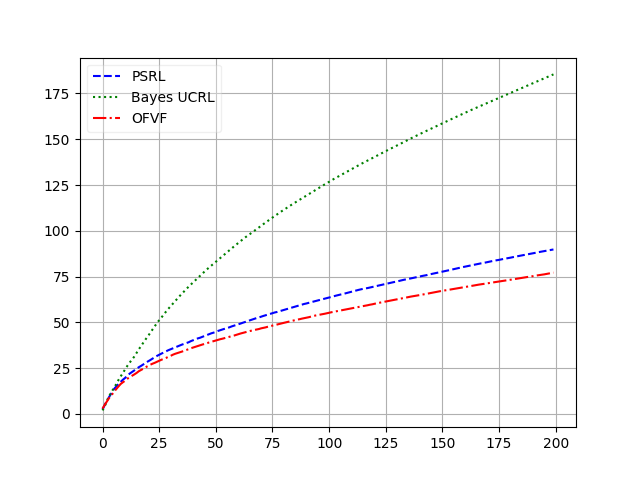
\includegraphics[width=\linewidth]{figures/SimpleProblem_PSRL_BayesUCRL_OFVF.png}
	\end{minipage}%
	\begin{minipage}[c]{.45\columnwidth}
		\centering
		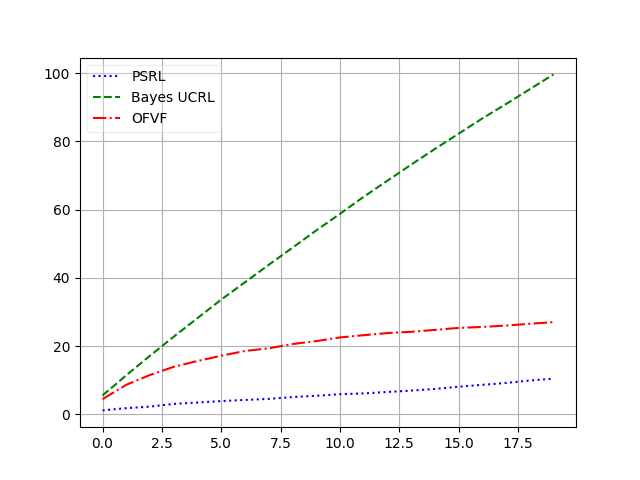
\includegraphics[width=\linewidth]{figures/RiverSwim_RSVF_BAYESUCB_PSRL.png}
	\end{minipage}%
	\caption{Cumulative regrets of PSRL and Bayes UCRL: left) above described simple problem, right) RiverSwim Problem described in \citep{Osband2013}}
	\label{fig:dirichlet_result}
\end{figure}

% \section{Some \LaTeX{} Examples}
% \label{sec:examples}

% \subsection{Sections}

% Use section and subsection commands to organize your document. \LaTeX{} handles all the formatting and numbering automatically. Use ref and label commands for cross-references.

% \subsection{Comments}

% You can add inline TODO comments with the todonotes package, like this:
% \todo[inline, color=green!40]{This is an inline comment.}

% \subsection{References}

% LaTeX automatically generates a bibliography in the APA style from your .bib file. The citep command generates a formatted citation in parentheses \citep{Lamport1986}. The cite command generates one without parentheses. LaTeX was first discovered by \cite{Lamport1986}.

% \subsection{Tables and Figures}

% Use the table and tabular commands for basic tables --- see Table~\ref{tab:widgets}, for example. You can upload a figure (JPEG, PNG or PDF) using the files menu. To include it in your document, use the includegraphics command as in the code for Figure~\ref{fig:frog} below.

% % Commands to include a figure:
% \begin{figure}
% \centering
% 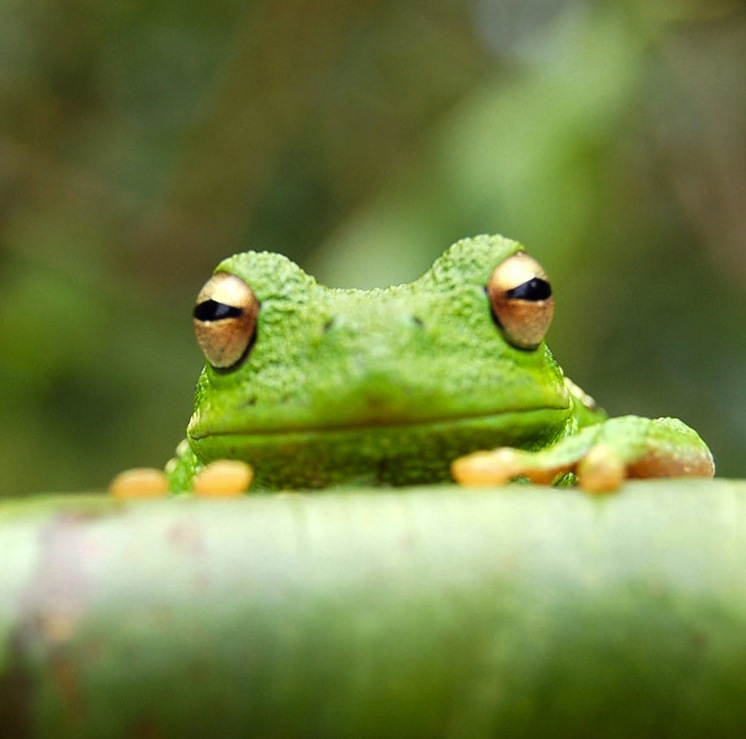
\includegraphics[width=0.5\textwidth]{frog.jpg}
% \caption{\label{fig:frog}This is a figure caption.}
% \end{figure}

% \begin{table}
% \centering
% \begin{tabular}{l|r}
% Item & Quantity \\\hline
% Widgets & 42 \\
% Gadgets & 13
% \end{tabular}
% \caption{\label{tab:widgets}An example table.}
% \end{table}

% \subsection{Mathematics}

% \LaTeX{} is great at typesetting mathematics. Let $X_1, X_2, \ldots, X_n$ be a sequence of independent and identically distributed random variables with $\text{E}[X_i] = \mu$ and $\text{Var}[X_i] = \sigma^2 < \infty$, and let
% $$S_n = \frac{X_1 + X_2 + \cdots + X_n}{n}
%       = \frac{1}{n}\sum_{i}^{n} X_i$$
% denote their mean. Then as $n$ approaches infinity, the random variables $\sqrt{n}(S_n - \mu)$ converge in distribution to a normal $\mathcal{N}(0, \sigma^2)$.

% \subsection{Lists}

% You can make lists with automatic numbering \dots

% \begin{enumerate}
% \item Like this,
% \item and like this.
% \end{enumerate}
% \dots or bullet points \dots
% \begin{itemize}
% \item Like this,
% \item and like this.
% \end{itemize}

% We hope you find write\LaTeX\ useful, and please let us know if you have any feedback using the help menu above.

% \bibliography{example}
\bibliography{reazullib}
\end{document}

%
% Please see the package documentation for more information
% on the APA6 document class:
%
% http://www.ctan.org/pkg/apa6
%